% UTF-8

% single-chapter commands
\documentclass[../main/thesis.tex]{subfiles}
\onlyinsubfile{\appendix}  % single-chapter command
\begin{document}


\chapter{Mathematische Konventionen}
\label{appx:mathsymbols}
% zu 4

\onetable{H}{

\begin{tabular}{|c|p{10.5cm}|}
\hline
\textbf{Symbol} & \textbf{Beschreibung} \\
\hline
$\equiv$ & leitet die Definition des linksseitigen Bezeichners ein \newline (z.~B. Definition durch eine Abfolge von Arbeitsschritten) \\
\hline
 &  \\
\hline
px & Pixel; Einheit für die kleinste rechteckige Fläche in gerasterter Darstellung, z.~B. auf dem Bildschirm; für \osm\ in der Regel quadratisch; bezeichnet als Einheit für eine Länge die Länge einer Pixelreihe von 1\,px Breite \\
\hline
\end{tabular}

\caption{Mathematische Abkürzungen und Symbole}
\label{tab:mathsymbols}
}
% TODO: neu (vgl. [Sar06])
...



\chapter{Bezeichner im Quelltext}
\label{appx:identifiers}
% zu 5.2

\onetable{H}{

\begin{tabular}{|p{3.3cm}|p{10.5cm}|}
\hline
\textbf{in Abschnitt~\ref{ch:algorithm-parts}} & \textbf{Entsprechung im Quelltext} \\
\hline
\textproc{Start} & Interface \texttt{Segment}, Methode \texttt{start} \\
\hline
\textproc{Ende} & \texttt{Segment.end} \\
\hline
\textproc{Segmentierung} & \texttt{Highway.segmentation} \\
\hline
\textproc{Splitten} & \texttt{SplitQueueIterator} \\
% SPLITTEN: SplitQueueIterator=S' (in Combiner.splitSegments), AbstractLine.splitCloseParallels()=für alle n/t, T enthält schon eine Parallitätsprüfung (warum? - in splitTargets/closeParallels)
\hline
\textproc{NaheSegmente} & \texttt{Combiner.regionaliseSegments} \\
% NAHESEGMENTE: Combiner.regionaliseSegments (arbeitet auf SourceSegments, also auf S statt S' und wurzel(s) statt s, weil so die Schnittmengenprüfung nicht wiederholt ausgeführt werden muss und damit ein Spatial Index erleichtert/ermöglicht wird)
\hline
\textproc{Hülle} & \texttt{SourceSegment.envelope} \\
\hline
\textproc{Fußpunkt} & \texttt{AbstractSegment.findPerpendicularFoot} \\
\hline
\textproc{Analyse} & \texttt{AbstractSegment.analyse} \\
\hline
\textproc{Parallel} & \texttt{SourceSegment.closeParallels} \\
% PARALLEL: SourceSegment.closeParallels / MyAnalyser
\hline
\textproc{Distanz} & \texttt{MyAnalyser.distance} \\
\hline
\textproc{NodesZuordnen} & \texttt{NodeGraph.createGraph} \\
\hline
\textproc{Zusammenfassen} & \texttt{GeneralisedLines.traverse} \\
\hline
\textproc{Generalisierung} & \texttt{Combiner.run} \\
\hline
\end{tabular}

\caption{Aufschlüsselung der Bezeichner in dieser Arbeit zu denen im Quelltext}
\label{tab:identifiers}
}

% TODO: Variablen innerhalb von ANALYSE und ZUSAMMENFASSEN ebenfalls aufschlüsseln?



\chapter{Datenmodell und Klassenstruktur}
\label{appx:fullpage-model}
% zu 5.3.2

\onefigure{ht}{
	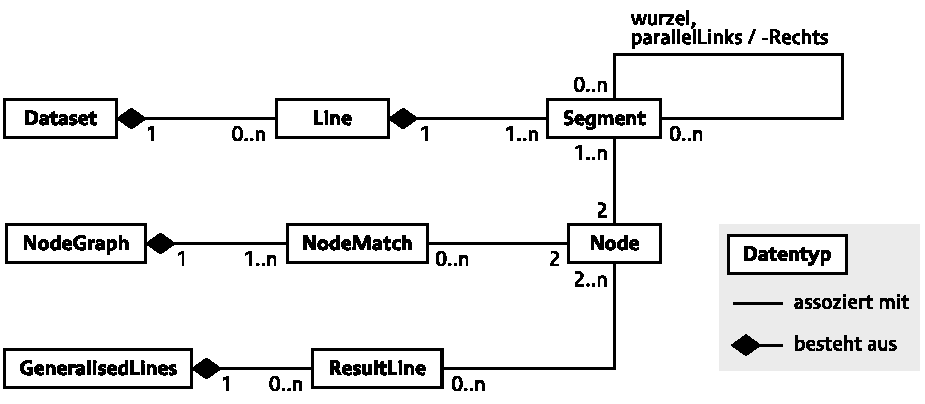
\includegraphics[scale=.69]{../appendices/data-model}
	\caption{Datenmodell}
	\label{fig:appx-data-model}
}

\onefigure{ht}{
	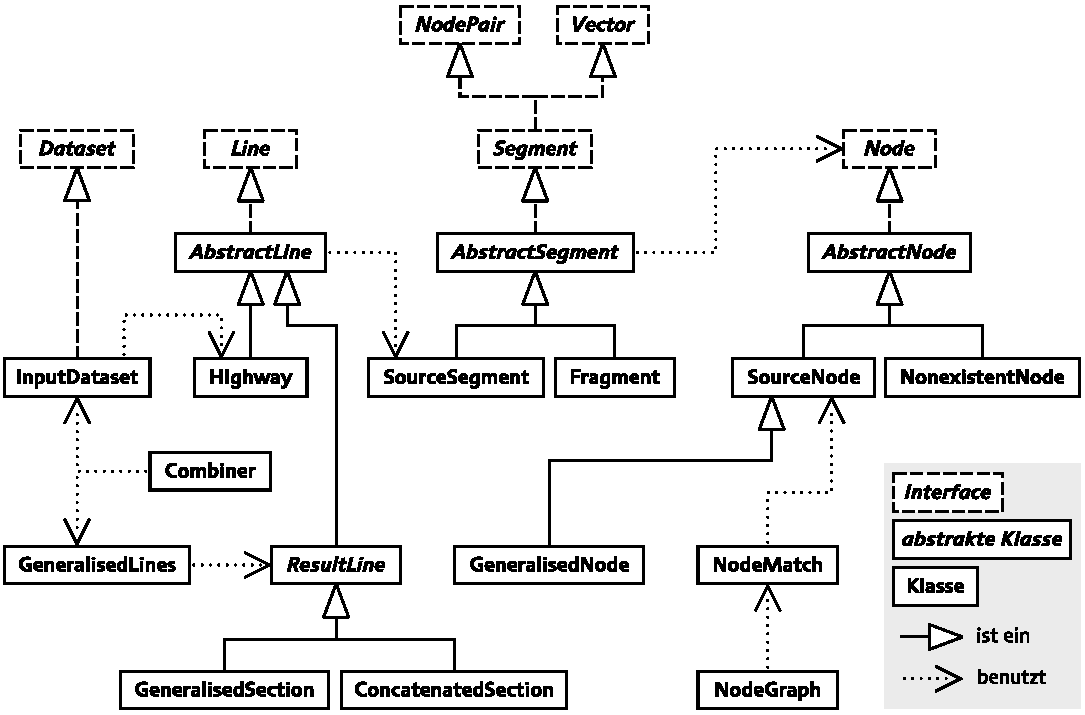
\includegraphics[scale=.69]{../appendices/class-structure}
	\caption
		[Klassenstrukturdiagramm für das Paket \code{comb}]
		{Klassenstrukturdiagramm für das Paket \code{comb} (aus Gründen der Übersichtlichkeit ist nur eine Auswahl der „benutzt“-Beziehungen dargestellt)}
	\label{fig:appx-class-structure}
}



\chapter{Anwendung auf ein Fernstraßennetz}
\label{appx:fullpage-examples-1}
% zu 6
% Beispiel für größeres Gebiet im Zusammenhang in kleinem Maßstab; evtl. unterschiedliche Regionen der Welt
% (Titel könnte sich noch ändern, vgl. E)

TBD



\chapter{Anwendung auf ein innerstädtisches Straßennetz}
\label{appx:fullpage-examples-2}
% zu 6
% Beispiel für größeres Gebiet im Zusammenhang in großem Maßstab; evtl. unterschiedliche Regionen der Welt
% (Titel könnte sich noch ändern, vgl. D)

TBD



\setcounter{chapter}{5}
\chapter{Beispiele für problematische Kreuzungssituationen}
\label{appx:junction-examples}
% zu 6

TBD\\
\\
(weitere Beispiele des Scheiterns an unterschiedlichen Kreuzungen; auch zeigen, wie \term{\_links} das Topologielückenproblem hierbei nicht lösen, sondern vergrößern)



%\chapter{Glossar}
%\chapter{Abkürzungsverzeichnis}
%\chapter{Software-Dokumentation}


% single-chapter commands
\end{document}
